\documentclass{article}

\usepackage[colorlinks, urlcolor=blue, linkcolor=red, citecolor=green]{hyperref}
\usepackage{fancyhdr} %设置页眉和页脚的
\usepackage{extramarks} %设置continue那玩意的
\usepackage{amsmath}
\usepackage{amsthm}
\usepackage{amsfonts}
\usepackage{tikz} %画线的
\usepackage[plain]{algorithm}
\usepackage{algpseudocode}
\usepackage{enumerate}

\usetikzlibrary{automata,positioning}

%表
\usepackage{booktabs}
\usepackage{multirow}
\usepackage{array}
\usepackage{caption}
\DeclareCaptionFont{heiti}{\heiti} %还可以定义其他的
\captionsetup{labelsep=space, font={small, bf}, skip=2pt} %space可以改成quad

%图
%*****************图片及其相关设置***************************
\usepackage{graphicx}
\graphicspath{{tupian/}}
\usepackage{subfigure}
% 导入tikz包
\usepackage{tikz}
\usetikzlibrary{math}

%*****************代码相关设置***************************
\usepackage{pythonhighlight}
\usepackage{listings}
\lstset{language=R,
    basicstyle=\small\ttfamily,
    otherkeywords={0,1,2,3,4,5,6,7,8,9},
    morekeywords={TRUE,FALSE},
    deletekeywords={data,frame,length,as,character},
    keywordstyle=\color{blue},
    backgroundcolor=\color[RGB]{245,245,244},
}
%
% Basic Document Settings
%

\topmargin=-0.45in
\evensidemargin=0in
\oddsidemargin=0in
\textwidth=6.5in
\textheight=9.0in
\headsep=0.25in

\linespread{1.1}

\pagestyle{fancy}
\lhead{\hmwkAuthorName}
\chead{\hmwkClass}
\rhead{\firstxmark}
\lfoot{\lastxmark}
\cfoot{\thepage}

\renewcommand\headrulewidth{0.4pt}
\renewcommand\footrulewidth{0.4pt}

\setlength\parindent{0pt}

%
% Create Problem Sections
%

\newcommand{\enterProblemHeader}[1]{
    \nobreak\extramarks{}{Project \arabic{#1} continued on next page\ldots}\nobreak{}
    \nobreak\extramarks{Project \arabic{#1} (continued)}{Project \arabic{#1} continued on next page\ldots}\nobreak{}
}

\newcommand{\exitProblemHeader}[1]{
    \nobreak\extramarks{Project \arabic{#1} (continued)}{Project \arabic{#1} continued on next page\ldots}\nobreak{}
    \stepcounter{#1}
    \nobreak\extramarks{Project \arabic{#1}}{}\nobreak{}
}

%\setcounter{secnumdepth}{0}
\newcounter{partCounter}
\newcounter{homeworkProblemCounter}
\setcounter{homeworkProblemCounter}{1}
\nobreak\extramarks{Project \arabic{homeworkProblemCounter}}{}\nobreak{}

\newenvironment{homeworkProblem}{
    \section{Project \arabic{homeworkProblemCounter}}
    \setcounter{partCounter}{1}
    \enterProblemHeader{homeworkProblemCounter}
}{
    \exitProblemHeader{homeworkProblemCounter}
}

%
% Homework Details
%   - Title
%   - Due date
%   - Class
%   - Section/Time
%   - Instructor
%   - Author
%

\newcommand{\hmwkTitle}{Project 2}
\newcommand{\hmwkDueDate}{May 18, 2021}
\newcommand{\hmwkClass}{Time Series Analysis}
\newcommand{\hmwkClassTime}{}
\newcommand{\hmwkClassInstructor}{Professor Tianwei Yu}
\newcommand{\hmwkAuthorName}{Peng Deng}
\newcommand{\hmwkAuthorSchool}{School of Data Science}
\newcommand{\hmwkAuthorNumber}{Sno.220041042}
%
% Title Page
%

\title{
    \vspace{2in}
    \textmd{\textbf{\hmwkClass: \hmwkTitle}}\\
    \normalsize\vspace{0.1in}\small{Due\ on\ \hmwkDueDate}\\
    \vspace{0.1in}\large{\textit{\hmwkClassInstructor\ \hmwkClassTime}}
    \vspace{3in}
}

\author{\textbf{\hmwkAuthorName}}


\date{}

\renewcommand{\part}[1]{\textbf{\large Part \Alph{partCounter}}\stepcounter{partCounter}\\}

%
% Various Helper Commands
%

% Useful for algorithms
\newcommand{\alg}[1]{\textsc{\bfseries \footnotesize #1}}
\usepackage[algo2e,vlined,ruled]{algorithm2e}

% For derivatives
\newcommand{\deriv}[1]{\frac{\mathrm{d}}{\mathrm{d}x} (#1)}

% For partial derivatives
\newcommand{\pderiv}[2]{\frac{\partial}{\partial #1} (#2)}

% Integral dx
\newcommand{\dx}{\mathrm{d}x}

% Alias for the Solution section header
\newcommand{\solution}{\textbf{\large Solution}}

% Probability commands: Expectation, Variance, Covariance, Bias
\newcommand{\E}{\mathrm{E}}
\newcommand{\Var}{\mathrm{Var}}
\newcommand{\Cov}{\mathrm{Cov}}
\newcommand{\Bias}{\mathrm{Bias}}
\begin{document}

\maketitle
\thispagestyle{empty}
\pagebreak
\thispagestyle{empty}
\tableofcontents

\newpage
\setcounter{page}{1}
\section{Problem statement}
Using the {\ttfamily getSymbols()} command in the R package {\ttfamily"quantmod"}, you can retrieve the stock price of Alibaba at New York Stock Exchange (NYSE) between 2015-01-01 and 2019-12-31. Please use the daily closing price to conduct the following analyses.
\begin{enumerate}[(1)]
    \item Explore the data. Comment on data characteristics. Is any transformation necessary?
    \item Try to fit an arima model to the data.
    \item Using the residual of the model you select from step 2, examine if there is change in variance over time. If the answer is yes, fit a model to describe the behavior of the residuals.
    \item Using the model from step 2, forecast the next month's data, and compare the forecast results to real data of 2020 .
    \item Using the differential data of the closing stock price, fit a Hidden Markov Model with 2 hidden states. Does there appear to be two distinct states?
    \item If you first take log of the price, observe the data and then repeat the analysis in $(5)$, does your conclusion change? Why? If there is any difference, which analysis do you think is more meaningful?
    \item Write a report to document your analysis and summarize your findings. Attach your code at the end of the report.
\end{enumerate}
\vspace{4pt}
\section{Data overview}

Firstly, we can have a quick look at the dataset, we plot the data as Figure \ref{dataset}. As we can see from Figure \ref{dataset}, there is not seasonal variation in the time series data, and the main trend of the data is increasing. 
More specifically, we can see that the trend in the first three years is increasing but not linear, and the data in the last two years changes dramatically. Thus, we can take \textbf{log transformation} to make the trend in the first three years more linear and to reduce the variation in the last two years. 
\begin{figure}[htbp]
    \centering
    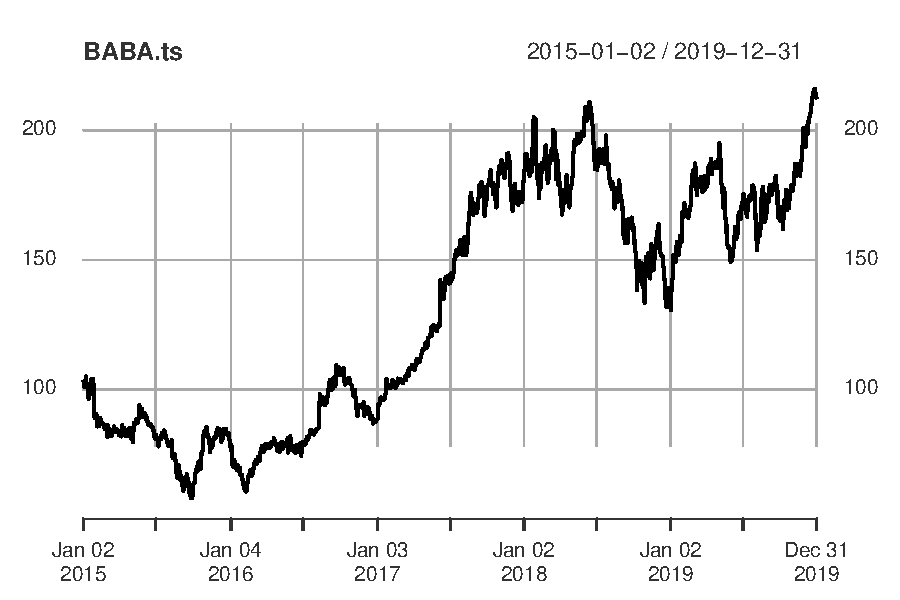
\includegraphics[width=0.6\linewidth]{images/dataset}
    \caption{The stock price of Alibaba between 2015-01-01 and 2019-12-31}
    \label{dataset}
\end{figure}
\vspace{4pt}
\section{Fit the ARIMA model and do forecast}
\label{sec3}
In this section, we would like to fit an ARIMA model to the stock price of Alibaba and do forecast.
\vspace{4pt}
\subsection{Fit the ARIMA model} 
In order to determine the parameters in ARIMA, we call ”auto.arima” in R as follow
\begin{lstlisting}[language=R]
BABA.arima = auto.arima(BABA.ts)
\end{lstlisting}
Then, we get the parameters of ARIMA is:
ARIMA(2,1,2). The fitted figures are as Figure \ref{BABA-arima-fit}.
\begin{figure}[htbp]
    \centering
    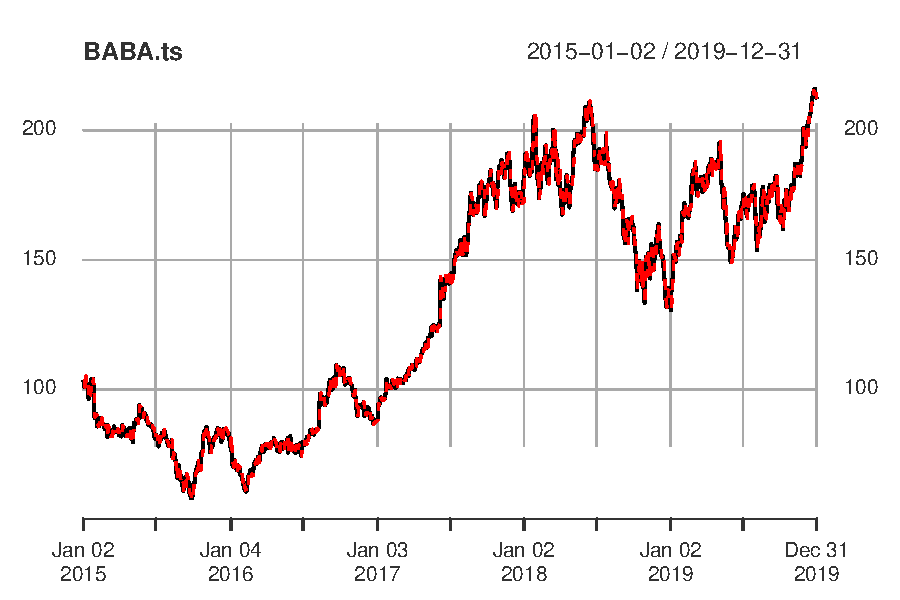
\includegraphics[width=0.6\linewidth]{images/BABA-arima-fit}
    \caption{ARIMA model fitted figure}
    \label{BABA-arima-fit}
\end{figure}

Then, we plot the residuals and the ACF figure of the residuals according to the ARIMA model result as Figure \ref{BABA-arima-res}, which means we are going to check residuals.
\begin{figure}[htbp]
    \centering
    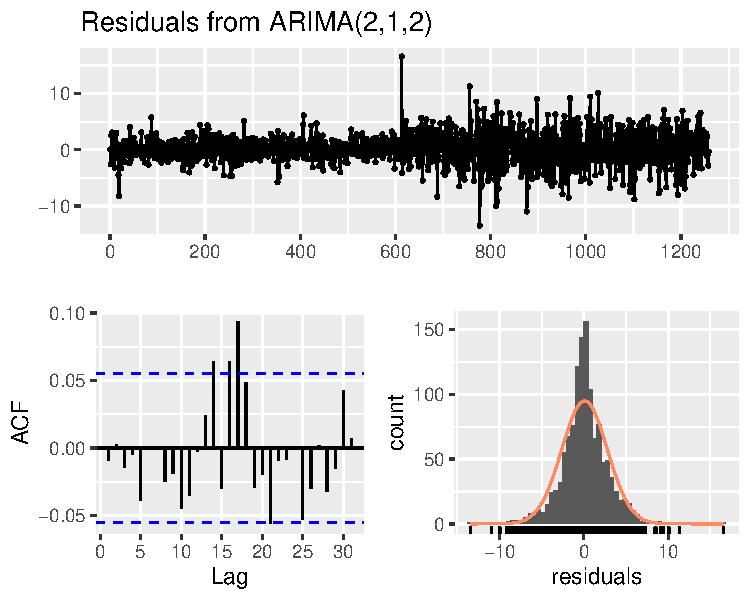
\includegraphics[width=0.7\linewidth]{images/BABA-arima-res}
    \caption{Check residuals of ARIMA model}
    \label{BABA-arima-res}
\end{figure}
As we can see from Figure \ref{BABA-arima-res}, there is significant acf, so that the model is not very good.  However, we can do the Ljung-Box test of the residuals to see if the residuals exhibit serial correlation, the result is as follow:
\begin{lstlisting}
	Ljung-Box test

data:  Residuals from ARIMA(2,1,2)
Q* = 6.0748, df = 6, p-value = 0.4149

Model df: 4.   Total lags used: 10
\end{lstlisting}
As we can see from the Ljung-Box test, the p-value equals 0.4149, which is larger than 0.05, so that we should not reject the null hypothesis, which means 
the residuals does not exhibit serial correlation. Thus, we can believe that the ARIMA model is suitable.
\vspace{4pt}
\subsection{Do the forecast}
Then, we would like to forecast the next month's data using the ARIMA model we fitted. As we can see from Figure \ref{BABA-arima-forecast}, the forecast is not 
good, and the value of the forecast is almost constant and it is far away from the true value. We zoom in the Figure \ref{forecast1} as Figure \ref{forecast2} in order to see clearly and do comparison.
Thus, maybe the ARIMA model is not good enough to do the forecast in this problem.

\begin{figure}[H]
    \centering
    \subfigure[The forecast]{\label{forecast1}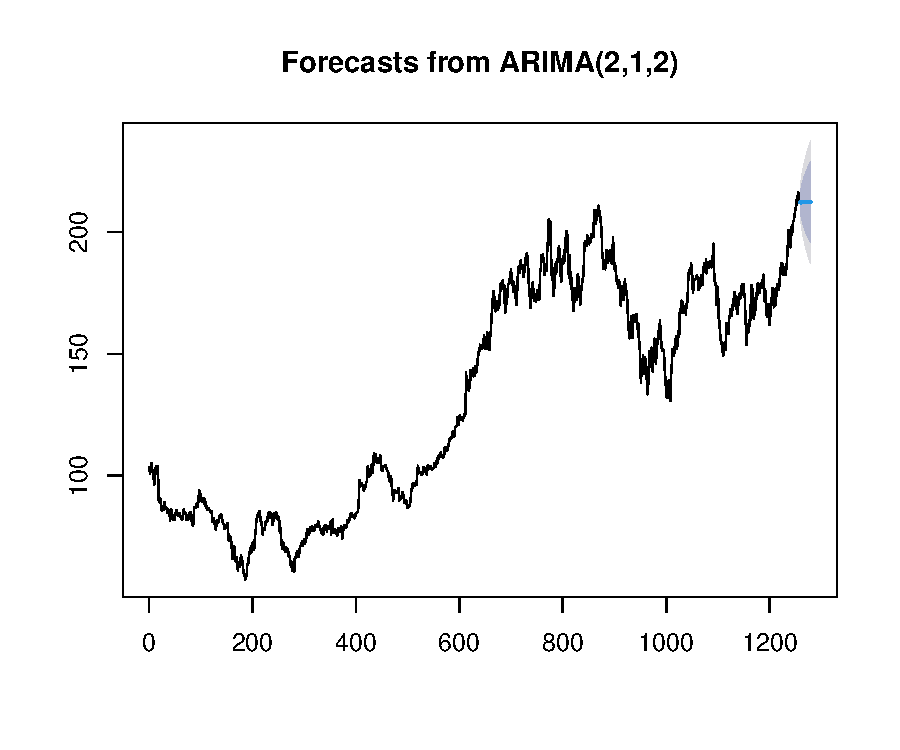
\includegraphics[width=0.48\linewidth]{images/BABA-arima-forecast}}
    \quad
    \subfigure[The comparison of forecast and true data]{\label{forecast2}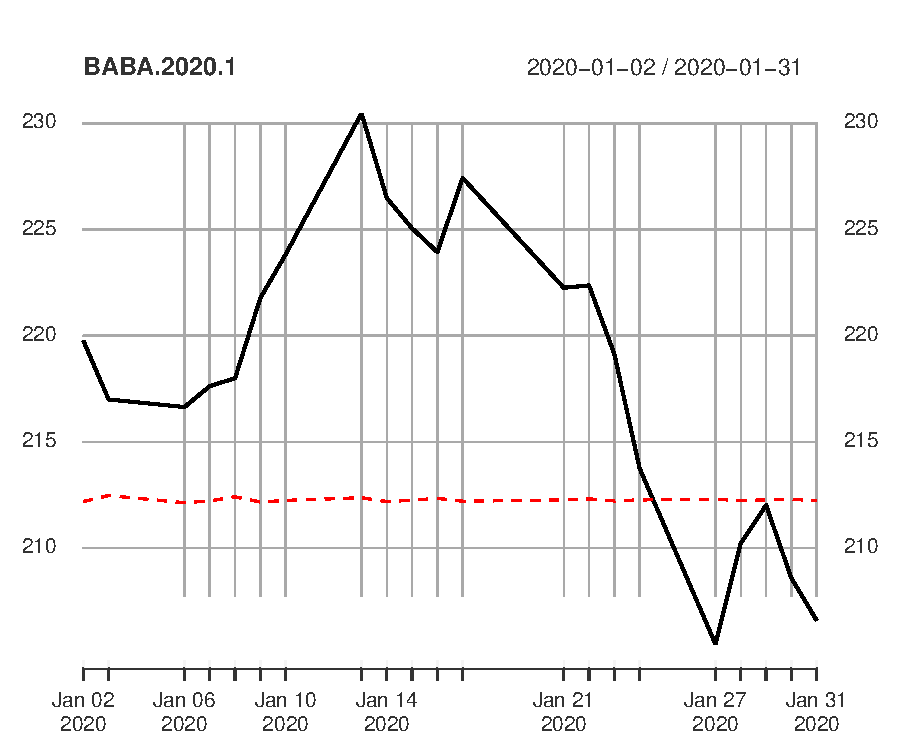
\includegraphics[width=0.48\linewidth]{images/BABA-forecast-2020.1}}
    \caption{The forecast of the next month}
    \label{BABA-arima-forecast}
\end{figure}

\vspace{4pt}
\section{Check the residuals}
In this section, we would like to deal with the residuals of the ARIMA model in Section \ref{sec3}.
\vspace{4pt}
\subsection{Examine the change in varaince}
As we can see from Figure \ref{BABA-arima-res}, the variance of residuals seems not constant over time. Then, we can plot the correlogram of the squared values to detect the volatility as Figure \ref{res-square}. As we can see, the variance is correlated in time, since the series exhibits volatility which can be derived from Figure \ref{res-sqaure2}. 
Thus, we can see that there is change in variance over time.
\begin{figure}[H]
    \centering
    \subfigure[The squared residuals]{\label{res-sqaure1}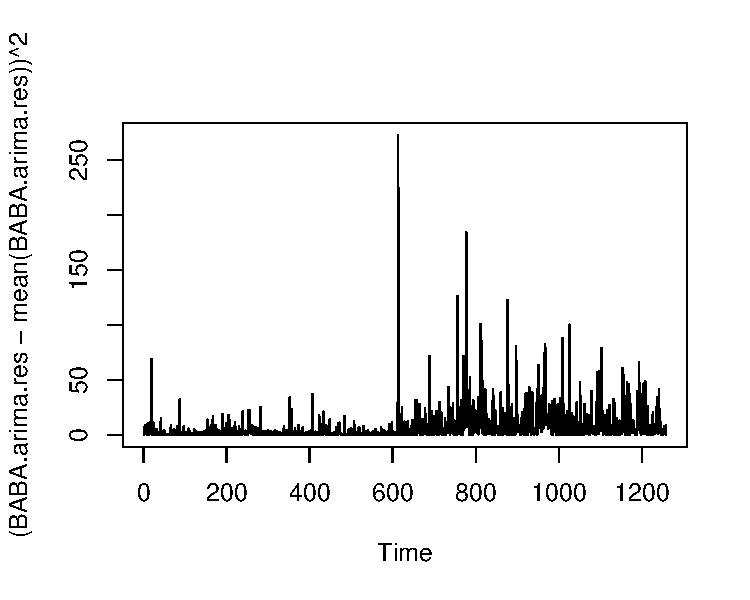
\includegraphics[width=0.48\linewidth]{images/BABA-res-square}}
    \quad
    \subfigure[The acf of the squared residuals]{\label{res-sqaure2}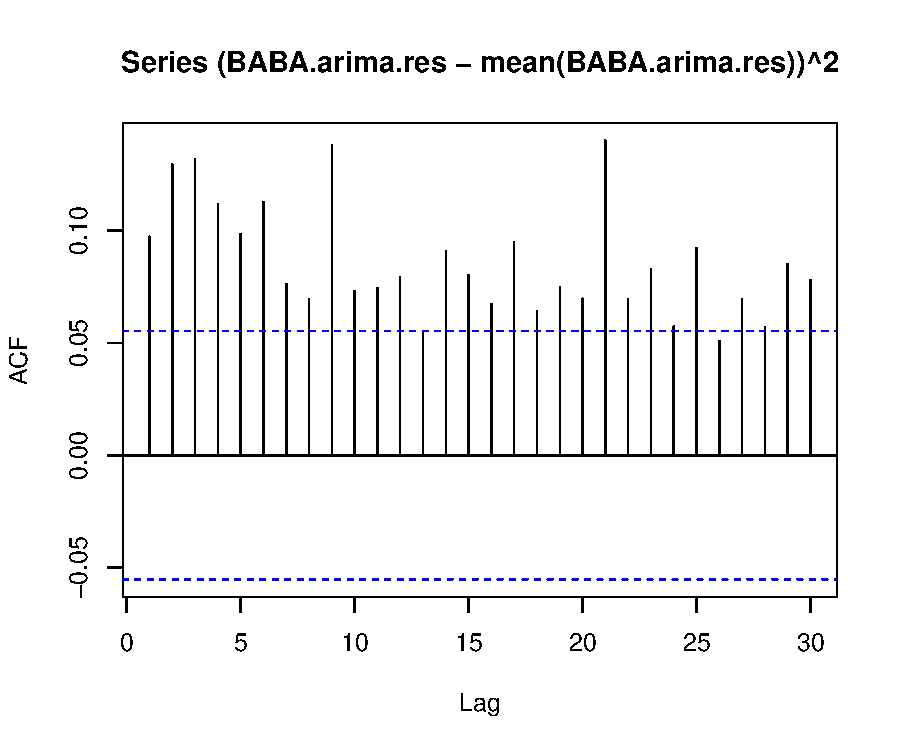
\includegraphics[width=0.48\linewidth]{images/BABA-res-acf}}
    \caption{The squared value of residuals time series}
    \label{res-square}
\end{figure}
\subsection{Fit the residuals}
We fit the residuals with GARCH(1,1) model, the series with fitteds standard deviation is as Figure \ref{BABA-res-garch-fit}. 
And the time sequence plot of the estimated conditional variance is as Figure \ref{BABA-res-con-variance}. 

\begin{figure}[H]
    \centering
    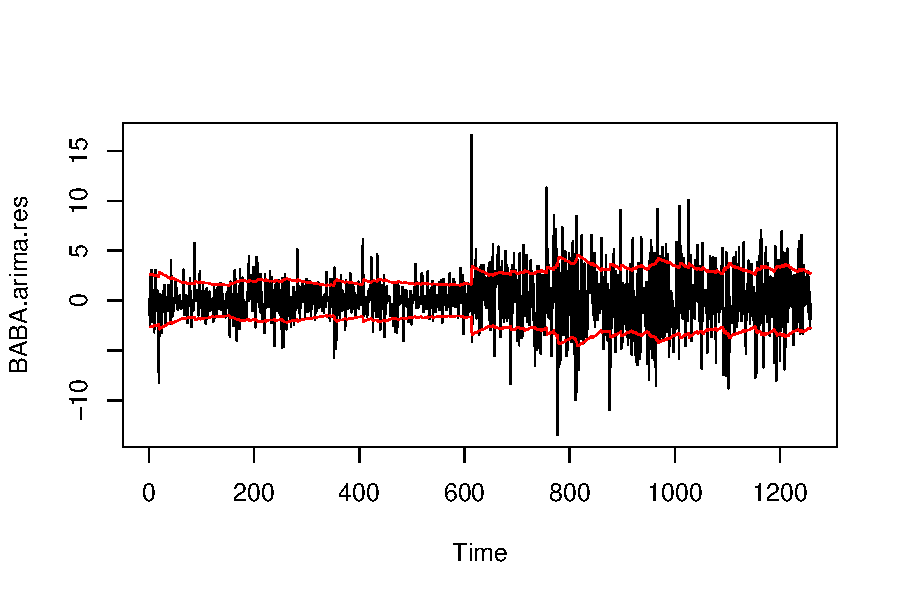
\includegraphics[width=0.7\linewidth]{images/BABA-res-garch-fit}
    \caption{The residuals with GARCH(1,1) model fitted standard deviation}
    \label{BABA-res-garch-fit}
\end{figure}

\begin{figure}[H]
    \centering
    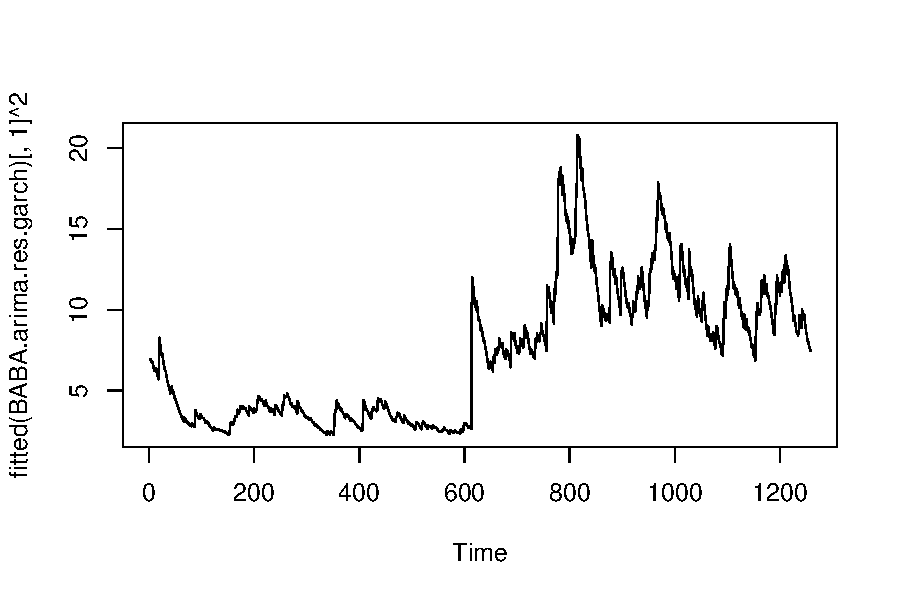
\includegraphics[width=0.7\linewidth]{images/BABA-res-con-variance}
    \caption{The time sequence plot of the estimated conditional variance}
    \label{BABA-res-con-variance}
\end{figure}
Then, we would like to check if the model have addressed the conditional heteroskedasticity. As we know, if all estimated conditional variance captures the conditional variance, the residuals will be white noise with mean 0 and variance 1.

\vspace{4pt}
Thus, we would like to check the residuals of GARCH(1,1) model. The test result is as follow and the test figures are as Figure \ref{BABA-res-garch-checkres}.
\begin{lstlisting}
Diagnostic Tests:
	Jarque Bera Test

data:  Residuals
X-squared = 4475.9, df = 2, p-value < 2.2e-16

	Box-Ljung test

data:  Squared.Residuals
X-squared = 0.11738, df = 1, p-value = 0.7319
\end{lstlisting}
As we can see from the Jarque Bera Test result, the $p$-value $<2.2e^{-16}$, which means the distribution of residuals is not normal. On the other hand, as we can see 
from the Box-Ljung test result, the $p$-value equals 0.7319, which means there is no serial autocorrelation in residuals. With the ACF figure of residuals in
Figure \ref{BABA-res-garch-checkres}, we ca derive that the residuals can be 
treated as white noise, which means the GARCH(1,1) model has addressed the conditional heteroskedasticity, although the distribution of residuals is not normal.

\begin{figure}[H]
    \centering
    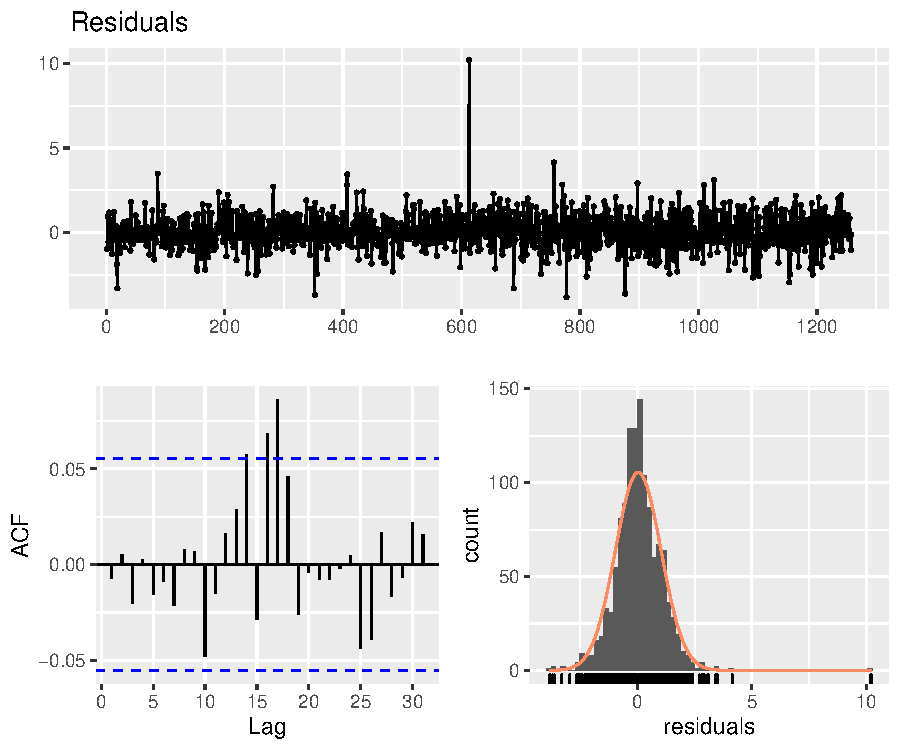
\includegraphics[width=0.7\linewidth]{images/BABA-res-garch-check-res}
    \caption{The time sequence plot of the estimated conditional variance}
    \label{BABA-res-garch-checkres}
\end{figure}

\section{HMM model}

\subsection{Do not take log to the original data}
Firstly, we would like to take differential to the closing stock price, the differential data of the closing stock price is showed as Figure \ref{differential}. 
As we can see from Figure \ref{differential}, it seems that there are two hidden states in the series.

\begin{figure}[H]
    \centering
    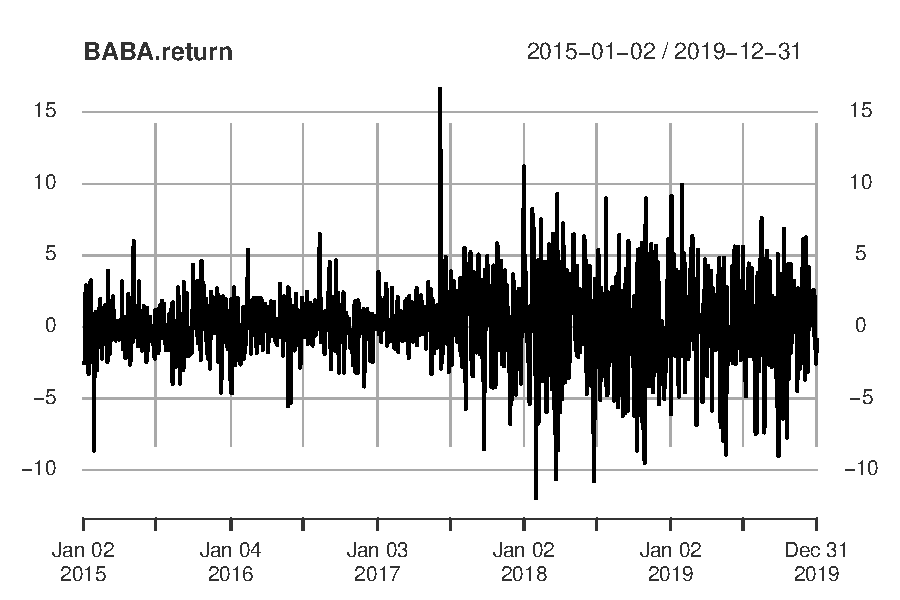
\includegraphics[width=0.7\linewidth]{images/differential}
    \caption{The differential data of the closing stock price}
    \label{differential}
\end{figure}
Then, we fit a Hidden Markov Model with 2 hidden states. The result is as Figure \ref{hmm}.
\begin{figure}[H]
    \centering
    \subfigure[The viterbi decoding]{\label{hmm1}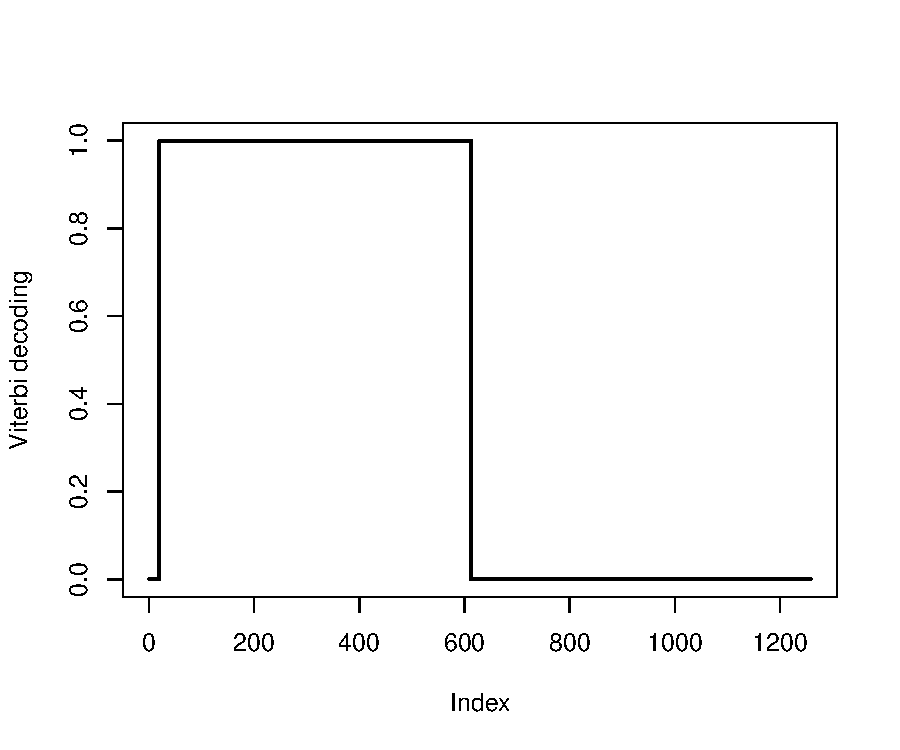
\includegraphics[width=0.48\linewidth]{images/hmm1}}
    \quad
    \subfigure[The posterior decoding]{\label{hmm2}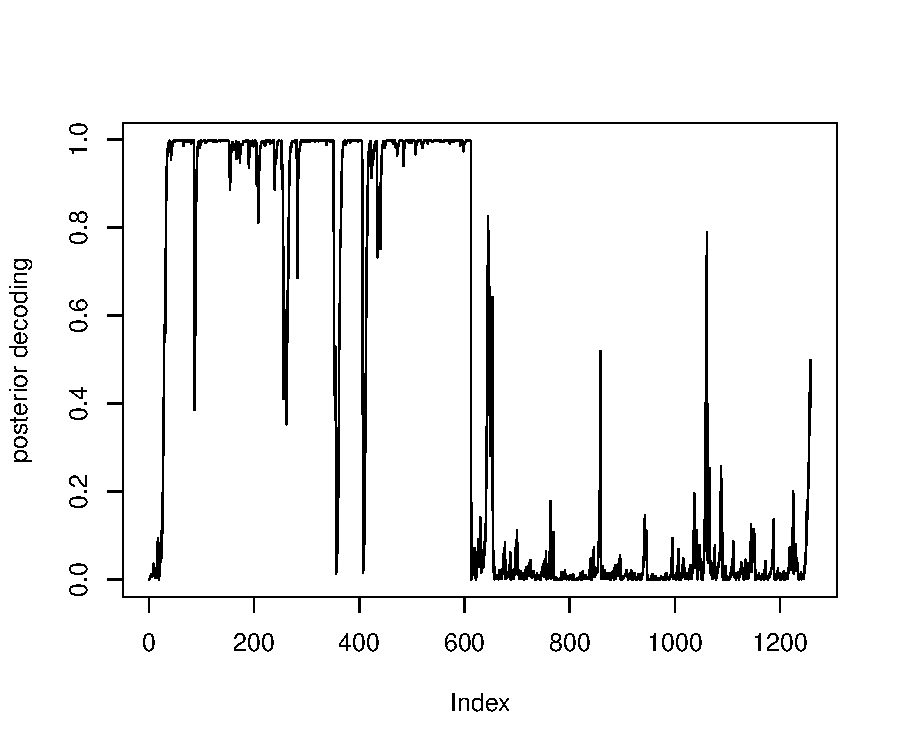
\includegraphics[width=0.48\linewidth]{images/hmm2}}
    \caption{The HMM model result}
    \label{hmm}
\end{figure}
As we can see from Figure \ref{hmm1}, the Viterbi decoding tells us there appear to be two distinct states, which meets our expectation as we mentioned before.
\subsection{Take log to the original data}
Firstly, we take log to the original price data, then the log price is as Figure \ref{BABA-log}.
\begin{figure}[H]
    \centering
    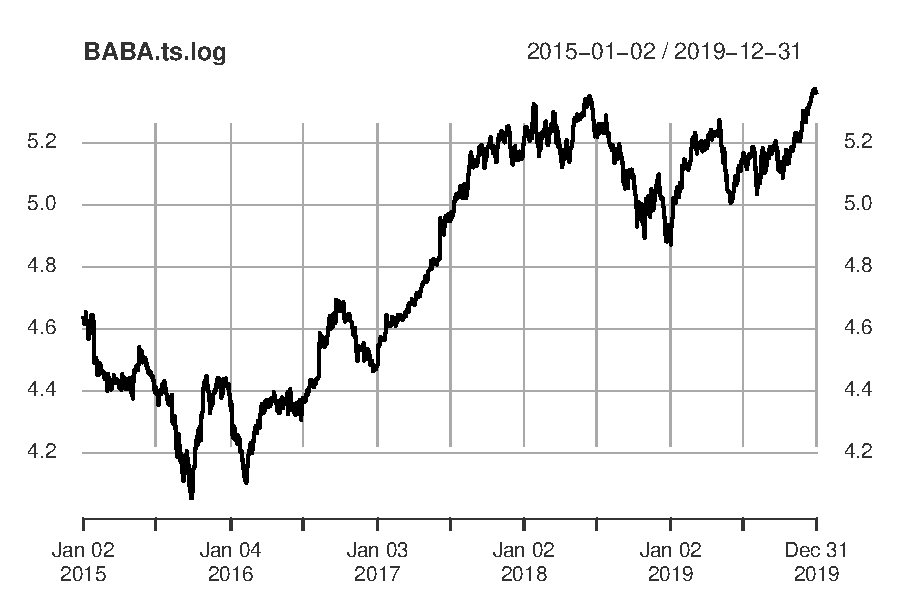
\includegraphics[width=0.7\linewidth]{images/BABA.log}
    \caption{The log data of the closing stock price}
    \label{BABA-log}
\end{figure}
Then, we again take differential to the log closing stock price, the differential data of the log closing stock price is showed as Figure \ref{differential2}. 
As we can see from Figure \ref{differential2}, it seems that there are not distinct hidden states in the series.

\begin{figure}[H]
    \centering
    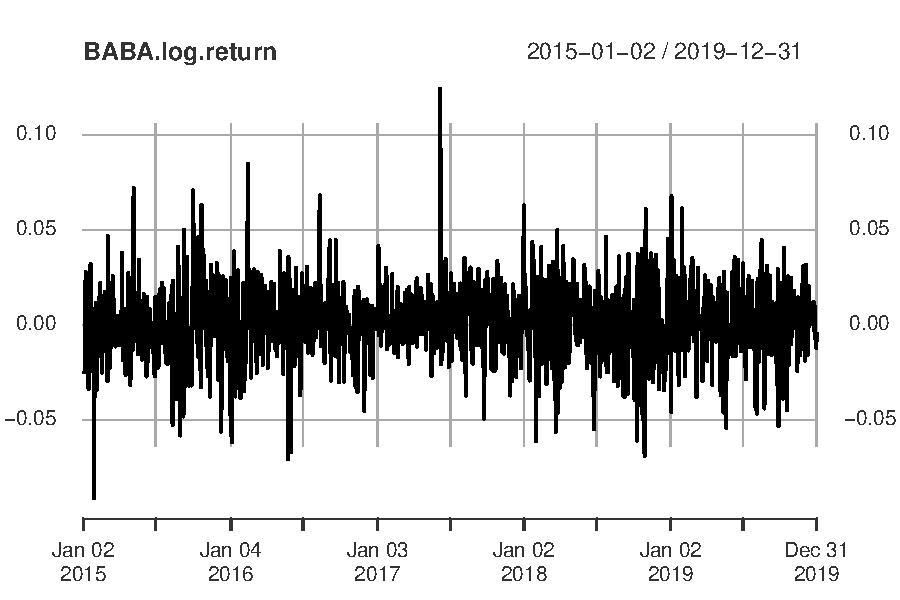
\includegraphics[width=0.7\linewidth]{images/differential2}
    \caption{The differential data of the log closing stock price}
    \label{differential2}
\end{figure}
Then, we fit a Hidden Markov Model with 2 hidden states. The result is as Figure \ref{hmm-log}.
\begin{figure}[H]
    \centering
    \subfigure[The Viterbi decoding]{\label{hmm-log1}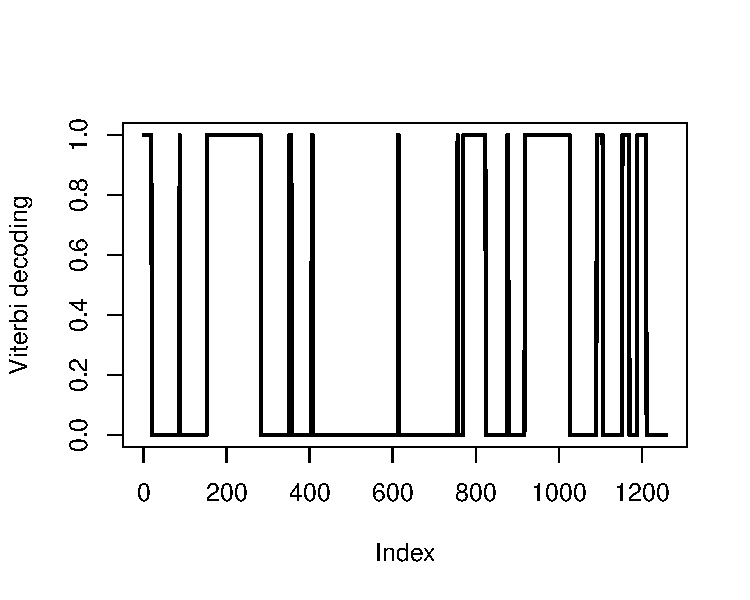
\includegraphics[width=0.48\linewidth]{images/hmm-log1}}
    \quad
    \subfigure[The posterior decoding]{\label{hmm-log2}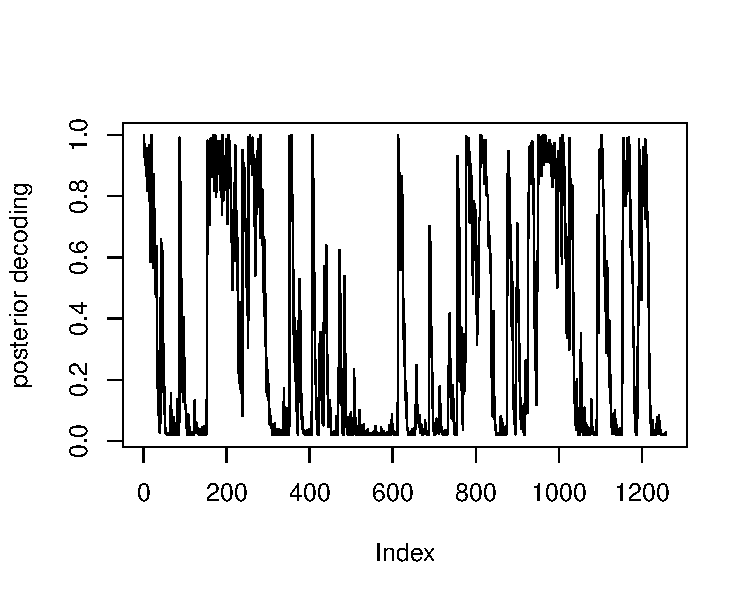
\includegraphics[width=0.48\linewidth]{images/hmm-log2}}
    \caption{The HMM model result}
    \label{hmm-log}
\end{figure}
As we can see from Figure \ref{hmm-log1}, there does not appear to have two distinct states because the viterbi decoding varies very frequently.

\vspace{4pt}
Thus, we can derive that after taking log to the original price data, the conclusion changes. There are no longer two distinct state is the return series. I think the analysis "Do not take log to the original data" is more meaningful, 
because in this analysis we can find two distinct states, which means the method is good to capture the feature of the original data.

\end{document}

